~\newpage
\nTitle{Programmation linéaire multicritère}

\section{Objectifs}
L'objectif est de trouver une solution de compromis entre les différents responsables.
Pour trouver une telle solution nous serons amenés à utiliser la programmation multicritère (\emph{PLM}).
Auparavant, dans la partie 1, nous avons trouvé un optimum pour chaque
responsable indépendam\-ment, ce qui nous conduit à un point de mire. Dans un
monde parfait, ce point de mire respecterait les contraintes de chaque
responsable. Nous devons donc voir si tel est le cas. 

\section{Recherche du point de départ}
Si le point de mire est assez proche de l'ensemble des solutions acceptables,
nous choisirons une solution proche de celle d'un responsable.

Sinon, nous allons calculer la satisfaction de chaque objectif, sachant qu'une
solution a été retenue. Nous devrons alors définir des métriques, correspondant
à cette satisfaction. Par exemple, pour le comptable, cette satisfaction sera
exprimée par le ratio du bénéfice obtenue dans un solution par rapport au
bénéfice maximal.
Ensuite, nous choisirons comme point de départ la solution qui offre le plus de
satisfaction à tout le monde, par exemple en utilisant une moyenne pondérée,
dont la pondération sera basée sur \emph{l'importance} de chaque critère.

\section{Affinement de la solution}
La solution trouvée précédemment peut sûrement être optimisée. Il peut être
intéressant de perdre dans un critère, si cela nous fait gagner beaucoup dans
un autre critère, d'autant plus si ce second critère est jugé plus
\emph{intéressant} que le premier.

\section{Métriques utilisées}
Cette section décrit les métriques utilisées pour caractériser une solution, du
point de vue d'un cadre de l'entreprise. Les solutions pourront ainsi être
comparées entre elles.

\paragraph{Comptable :}
La métrique utilisée sera le pourcentage du bénéfice par rapport au bénéfice
maximum :
$$
M_{Comptable} = \frac{B_{S}}{B_{max}} \times 100
$$

\paragraph{Responsable d'atelier}
La métrique utilisée sera le pourcentage du nombre de produits fabriqués par
rapport au nombre maximum :
$$
M_{Atelier} = \frac{N_{S}}{N_{max}} \times 100
$$

\paragraph{Responsable des stocks}
Pour élaborer la métrique de satisfaction pour le responsable des stocks nous
opterons pour la fonction suivante, qui correspond à ce qui était précédemment
annoncé dans la partie 1 (page \pageref{stocks}).

\begin{figure}[!ht]
\begin{center}
    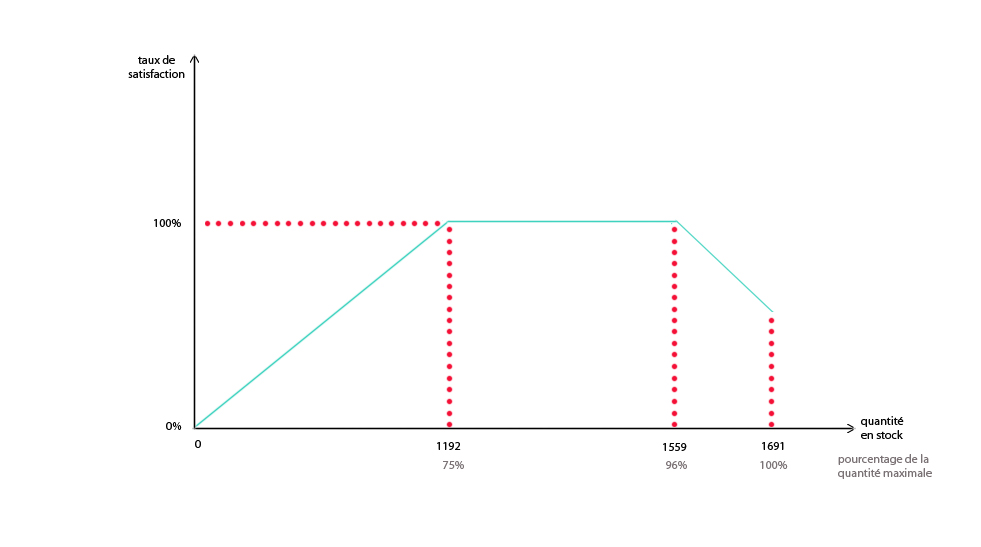
\includegraphics[width=\linewidth]{multicritere_graphe_stocks.png}
    \caption{Représentation graphique de la métrique pour le responsable des
	stocks.}
	\end{center}
\end{figure}

Cette fonction est décrite par l'expression suivante :
$$
M_{Stocks} = \left\{ 
    \begin{array}{l l l}
	\frac{x}{1192} \text{ si } x \in \text{[0 ; 1192]} \\
	x=1 \text{ si } x \in [1192 ; 1559]\\
	\frac{-x}{1192}+ 1+\frac{1559}{1192} \text{ si } x \in \text{[1559 ;
	    1691]}\\
    \end{array}
\right.
$$

Cette fonction pourrait être justifiée par le fait que plus on s’éloigne des
valeurs admises moins le responsable des stocks est satisfait.


\paragraph{Responsable commercial}
La métrique utilisée sera l'écart par rapport à un équilibre parfait.
Si autant de produit de la famille de produit 1 (comprenant les produits A, B
et C) que de la famille 2 (comprenant les produits D, E et F), la métrique sera
à 100\%.
Si une seule famille de produit est fabriquée, la métrique devra valoir zéro.

Si $F_1$ (respectivement $F_2$ est le nombre de produit de la famille 1
(respectivement famille 2), la métrique sera :
$$
M_{Commercial} = \left( 1 - \frac{|F_1 - F_2|}{F_1 + F_2} \right) \times 100
$$

\section{Utilisation}
Les résultats seront placés dans un tableau de ce type, qui qui permettra d'un
seul coup d'œil de voir la meilleur des solutions.
La colonne en rouge se lira par exemple : 
\begin{center}
«~En suivant la volonté du responsable d'atelier, le comptable aura une
satisfaction de $96.5498\%$~»
\end{center}

\begin{table}[!ht]
    \begin{center}
    \begin{tabular}{|l|c|c|c|c|}
\hline
\cellcolor[gray]{0.9} & Comptable& Atelier & Stock & Commercial  \\
\hline
Comptable			& \cellcolor[gray]{0.9} 100\% & 94.7678\% & 40.0930\%			  & 11.4302\% \\
\hline
Atelier				& \cellcolor{red}   96.5498\% &
\cellcolor[gray]{0.9} 100\% & 32.2825\%			  & 47.9244\% \\
\hline
Stock			        & 74.1546\%		      & 70.8003\%		    & \cellcolor[gray]{0.9} 100\% & 25.2908\% \\
\hline
Commercial			& 81.8654\%		      & 93.4330\%
& 30.6085\%                   & \cellcolor[gray]{0.9} 100\% \\
\hline
    \end{tabular}
    \end{center}
    \caption{Tableau de satisfaction des différents cadres de l'entreprise en
	fonction de la solution retenue.}
\end{table}

On voit bien que le point de mire est éloigné de l'ensemble des solutions
acceptables : aucune solution ne semble satisfaire tous les responsables.

\section{Optimisation}
Nous allons dans cette partie essayer de modifier les solutions précédentes
pour trouver une solution qui tente de maximiser la satisfaction des différents
responsables.

Le but premier d'une entreprise étant de faire du profit, et la meilleur manière de
faire du profit étant souvent maximiser le bénéfice, nous allons donc favoriser
ce critère, en lui appliquant un léger coefficient.

Nous allons par la même regarder l'évolution des autres critères lorsque ce
coefficient évolue, c'est à dire recalculer les différentes métriques.

Il apparaît plausible qu'avoir un \emph{stock non optimal} peut être acceptable
si c'est pour avoir un bénéfice plus important, dans une certaine mesure. Une
dégradation de la satisfaction du responsable des stock sera donc moins
pénalisant, en terme de qualité de solution, qu'une baisse dans la satisfaction
du commercial (produire sans vendre ne sert pas à grand chose, en terme de
rentabilité).

De la même manière, produire un nombre de produit optimal peut être
intéressant, mais cela ne doit pas aller à l'encontre du profit et de la
mauvaise répartition de la production.

Nous pouvons donc donner des coefficients aux critères :

\begin{table}[h!]
\begin{center}
\begin{tabular}{|l||c|c|c|c|}
\hline
    Responsable & Comptable & Atelier & Commercial & Stocks \\
	\hline
    Coefficient & 1.2	    & 0.8     & 1.2	& 0.8 \\
	\hline
	\end{tabular}
	\end{center}
\caption{Coefficient associés aux critères des différents responsables}
\end{table}

\subsection{Méthodologie d'optimisation}
Le procédé sera itératif, et partira de la solution du comptable. 
\subsection{Résultats}
Présenter un tableau.
